\documentclass[a4paper,twoside]{article}
\usepackage[T1]{fontenc}
\usepackage[bahasa]{babel}
\usepackage{graphicx}
\usepackage{graphics}
\usepackage{float}
\usepackage[cm]{fullpage}
\pagestyle{myheadings}
\usepackage{etoolbox}
\usepackage{setspace} 
\usepackage[dvipsnames]{xcolor}
\usepackage{lipsum} 
\usepackage{xspace}
\usepackage{hyperref}
\setlength{\headsep}{30pt}
\usepackage[inner=2cm,outer=2.5cm,top=2.5cm,bottom=2cm]{geometry} %margin
% \pagestyle{empty}

\hypersetup{colorlinks=true,urlcolor=SkyBlue,linkcolor=MidnightBlue}

\makeatletter
\renewcommand{\@maketitle} {\begin{center} {\LARGE \textbf{ \textsc{\@title}} \par} \bigskip {\large \textbf{\textsc{\@author}} }\end{center} }
\renewcommand{\thispagestyle}[1]{}
\markright{\textbf{\textsc{AIF184001/AIF184002 \textemdash Rencana Kerja Tugas Akhir \textemdash Sem. Genap 2024/2025}}}

\newcommand{\HRule}{\rule{\linewidth}{0.4mm}}
\newcommand{\web}{\textit{web}\xspace}
\renewcommand{\baselinestretch}{1}
\setlength{\parindent}{0 pt}
\setlength{\parskip}{6 pt}

\onehalfspacing

\begin{document}
	
	\title{\@judultopik}
	\author{\nama \textendash \@npm} 
	
	%tulis nama dan NPM anda di sini:
	\newcommand{\nama}{Alfonsus Oktario Sutomo}
	\newcommand{\@npm}{6181801010}
	\newcommand{\@judultopik}{Perkembangan Penggunaan Teknologi Pembangunan Web Dunia} % Judul/topik anda
	\newcommand{\jumpemb}{1} % Jumlah pembimbing, 1 atau 2
	\newcommand{\tanggal}{19/02/2025}
	
	% Dokumen hasil template ini harus dicetak bolak-balik !!!!
	
	\maketitle
	
	\pagenumbering{arabic}
	
	\section{Deskripsi}
Perkembangan teknologi pembuatan \web telah mengalami perubahan yang sangat pesat dalam 60 bulan terakhir. Sejak kemunculannya, \web telah menjadi platform utama dalam penyebaran informasi, komunikasi, hingga transaksi digital. Seiring meningkatnya kebutuhan pengguna terhadap kecepatan, keamanan, dan interaktivitas, berbagai teknologi baru terus bermunculan untuk mendukung pengembangan \web yang lebih efisien dan responsif.

Internet sendiri merupakan jaringan yang menghubungkan berbagai perangkat untuk memungkinkan pertukaran informasi secara cepat. Pertukaran informasi ini diatur oleh protokol utama TCP/IP (\textit{Transmission Control Protocol/Internet Protocol}). Namun, informasi yang dikirimkan di internet harus mudah dipahami oleh pengguna, tidak hanya dalam bentuk teks tetapi juga melalui gambar, video, dan suara. Kebutuhan inilah yang mendorong berkembangnya layanan \web (\textit{World Wide \web}), yang memungkinkan penyajian informasi secara lebih interaktif dengan memanfaatkan protokol HTTP (\textit{HyperText Transfer Protocol}).

Teknologi pembuatan \web semakin beragam dalam perkembangannya, baik dari sisi \textit{front-end} maupun \textit{back-end}. Beberapa teknologi utama yang mendukung pengembangan \web di antaranya adalah JavaScript, PHP, dan MySQL. Munculnya berbagai \textit{framework} dan pustaka seperti React, Vue.js, dan Node.js juga mempercepat adopsi teknologi baru dalam pengembangan \web modern. Perubahan ini membuat pentingnya pemantauan tren teknologi \web agar pengembang dapat memilih teknologi yang sesuai dengan kebutuhan pengguna dan standar industri.

Situs \textit{HTTP Archive} menyediakan data tentang teknologi yang digunakan dalam pembuatan \web untuk mencatat perkembangannya. Situs ini mengumpulkan data berdasarkan berbagai aspek, seperti pengalaman pengguna dalam mengakses \web, kecepatan pemuatan halaman, serta tingkat aksesibilitas. Salah satu aspek utama yang diamati dalam penelitian ini adalah \textit{Chrome User Experience Report} (CrUX), yang mengukur tingkat interaktivitas dan kecepatan pemuatan \web berdasarkan data nyata dari pengguna peramban Google Chrome.

Data dari \textit{HTTP Archive} kemudian disimpan dalam \textit{Google BigQuery}, layanan penyimpanan dan analisis data berbasis \textit{cloud} yang memungkinkan pemrosesan data dalam skala besar menggunakan \textit{query SQL}. Dengan adanya teknologi ini, analisis terhadap perkembangan teknologi pembuatan \web dapat dilakukan secara lebih mendalam dan berbasis data yang akurat.

Untuk mempermudah pemahaman terhadap hasil analisis, penelitian ini akan menggunakan visualisasi data dalam bentuk grafik. Salah satu bentuk visualisasi yang digunakan adalah \textit{line chart}, yang dapat menunjukkan tren perubahan teknologi dalam rentang waktu tertentu secara lebih jelas. Contoh \textit{line chart} dapat dilihat pada gambar~\ref{fig:contohlinechart}.
%\footnote{Gambar didapatkan dari \url{https://www.simonsezit.com/article/how-to-make-a-line-graph-in-excel/}}. 
Perkembangan penggunaan berbagai teknologi \web dapat divisualisasikan sehingga pola-pola perubahan dapat dikenali dengan lebih mudah dengan menggunakan \textit{line chart}. Selain itu, bentuk visualisasi lainnya seperti \textit{bar chart} dan \textit{scatter plot} juga dapat digunakan untuk memberikan perspektif tambahan terhadap data yang dianalisis.

\begin{figure}[]
        \centering
        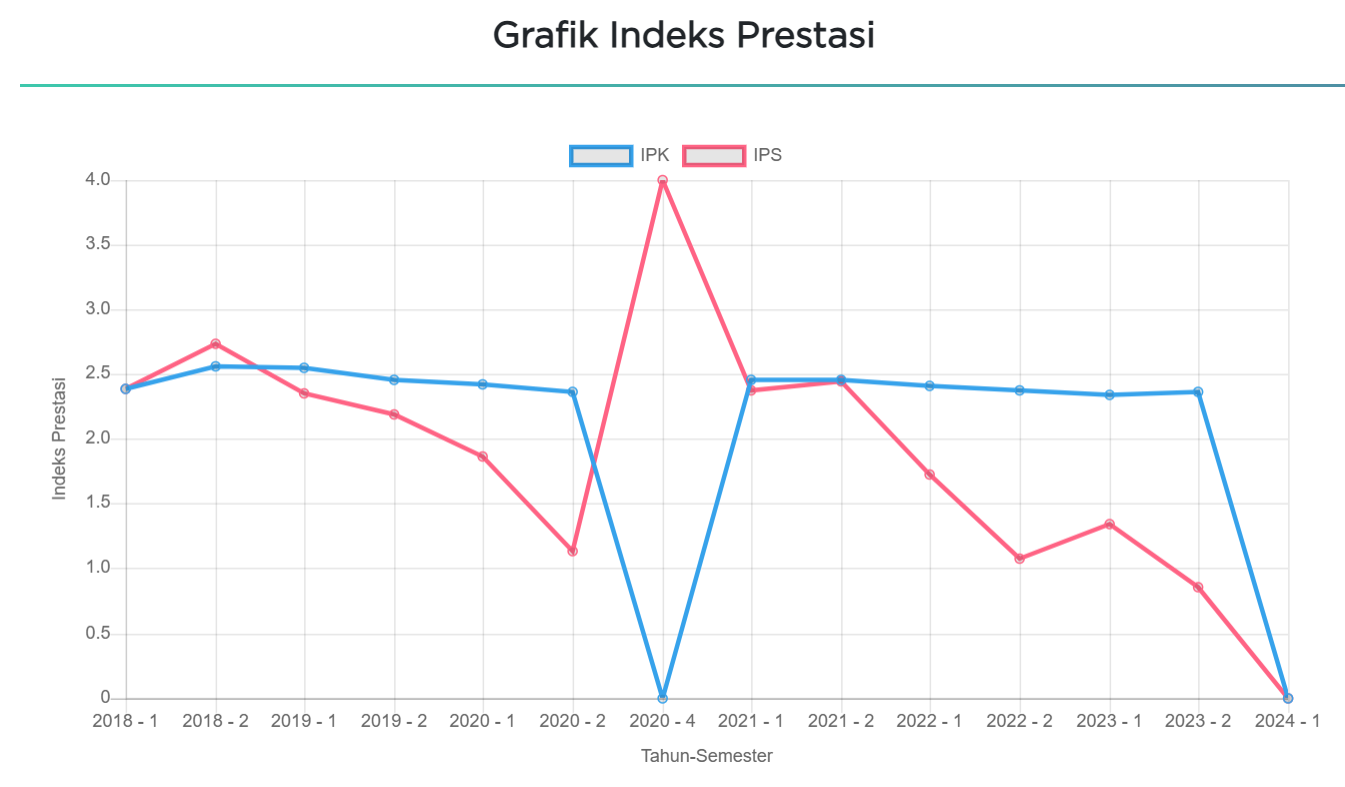
\includegraphics[width=0.5\linewidth]{Gambar/ContohLineChart.png}
        \caption{Contoh \textit{line chart}}
        \label{fig:contohlinechart}
    \end{figure}

Penelitian ini bertujuan untuk memahami bagaimana tren teknologi pembuatan \web berkembang dalam 60 bulan terakhir, dari Oktober 2018 hingga Desember 2024. Dengan menggunakan data dari \textit{HTTP Archive} dan \textit{Google BigQuery}, penelitian ini akan mengeksplorasi perubahan signifikan dalam penggunaan teknologi \web dan dampaknya terhadap pengalaman pengguna. Hasil analisis ini diharapkan dapat memberikan wawasan bagi pengembang \web dan industri teknologi dalam memahami arah perkembangan \web di masa depan.
	
	\section{Rumusan Masalah}
	Rumusan masalah yang akan diselesaikan dalam penelitian ini adalah:
    \begin{enumerate}
        \item Bagaimana perkembangan teknologi pembuatan \web selama 60 bulan terakhir?
        \item Bagaimana pekembangan teknologi pembuatan \web yang banyak digunakan oleh pembuat \web?
        \item Bagaimana cara menyajikan pekembangan teknologi pembuatan \web kepada pengguna?
    \end{enumerate}
	
	\section{Tujuan}
	Tujuan dari penelitian ini adalah:
    \begin{enumerate}
        \item Mengetahui perkembangan teknologi pembuatan \web selama 60 bulan terakhir.
        \item Mengetahui perkembangan teknologi pembuatan \web yang banyak digunakan oleh pembuat \web.
        \item Membuat perangkat lunak untuk menyajikan perkembangan teknologi pembuatan \web.
    \end{enumerate}
	
	\section{Deskripsi Perangkat Lunak}
	Perangkat lunak akhir yang akan dibuat memiliki fitur minimal sebagai berikut:
	\begin{itemize}
		\item Pengguna dapat melihat hasil perkembangan penggunaan teknologi pembuatan \web
		\item Pengguna dapat menentukan teknologi yang ingin dilihat  
		\item Pengguna dapat mengatur rentang waktu data yang ingin dilihat
		\item Pengguna dapat mengatur jenis data yang ingin dilihat dapat berdasarkan jumlah atau persentase dari teknologi yang digunakan
	\end{itemize}
	
	\section{Detail Pengerjaan Tugas Akhir}
	Bagian-bagian pekerjaan skripsi ini adalah sebagai berikut :
	\begin{enumerate}
		\item Melakukan studi literatur mengenai teknologi pembuatan \web
		\item Melakukan studi literatur mengenai bahasa SQL
            \item Melakukan studi literatur mengenai statistika
		\item Melakukan studi literatur mengenai visualisasi data
		\item Mempelajari penggunaan \textit{Google Big Query}
		\item Melakukan pengumpulan data perkembangan teknologi pembuatan \web
		\item Melakukan analisa dan visualisasi terhadap data perkembangan teknologi pembuatan \web
		\item Membangun perangkat lunak yang menampilkan hasil analisis dengan fitur yang interaktif 
		\item Menulis dokumen tugas akhir.
	\end{enumerate}
	
	\section{Rencana Kerja}
	Rincian capaian yang direncanakan di Tugas Akhir 1 adalah sebagai berikut:
	\begin{enumerate}
            \item Melakukan studi literatur mengenai teknologi pembuatan \web
		\item Melakukan studi literatur mengenai bahasa SQL
            \item Melakukan studi literatur mengenai statistika
		\item Melakukan studi literatur mengenai visualisasi data
		\item Mempelajari penggunaan \textit{Google Big Query}
            \item Menulis dokumen tugas akhir
	\end{enumerate}
	
	Sedangkan yang akan diselesaikan di Tugas Akhir 2 adalah sebagai berikut:
	\begin{enumerate}
            \item Melakukan pengumpulan data perkembangan teknologi pembuatan \web
		\item Melakukan analisa dan visualisasi terhadap data perkembangan teknologi pembuatan \web
		\item Membangun perangkat lunak yang menampilkan hasil analisis dengan fitur yang interaktif 
		\item Menulis dokumen tugas akhir.
	\end{enumerate}
	
	\vspace{1cm}
	\centering Bandung, \tanggal\\
	\vspace{2cm} \nama \\ 
	\vspace{1cm}
	
	Menyetujui, \\
	\ifdefstring{\jumpemb}{2}{
		\vspace{1.5cm}
		\begin{centering} Menyetujui,\\ \end{centering} \vspace{0.75cm}
		\begin{minipage}[b]{0.45\linewidth}
			% \centering Bandung, \makebox[0.5cm]{\hrulefill}/\makebox[0.5cm]{\hrulefill}/2013 \\
			\vspace{2cm} Nama: \makebox[3cm]{\hrulefill}\\ Pembimbing Utama
		\end{minipage} \hspace{0.5cm}
		\begin{minipage}[b]{0.45\linewidth}
			% \centering Bandung, \makebox[0.5cm]{\hrulefill}/\makebox[0.5cm]{\hrulefill}/2013\\
			\vspace{2cm} Nama: \makebox[3cm]{\hrulefill}\\ Pembimbing Pendamping
		\end{minipage}
		\vspace{0.5cm}
	}{
		% \centering Bandung, \makebox[0.5cm]{\hrulefill}/\makebox[0.5cm]{\hrulefill}/2013\\
		\vspace{2cm} Pascal~Alfadian,~Nugroho,~M.Comp.\\ Pembimbing Tunggal
	}
\end{document}
